\documentclass[10pt,letterpaper]{article}
\usepackage[margin=0.65in]{geometry}
\usepackage{amsmath,amssymb,mathtools,graphicx,booktabs,array,xcolor,fancyhdr,hyperref}
\definecolor{ink}{HTML}{0B3A6B}
\definecolor{pale}{HTML}{F4F8FB}
\pagestyle{fancy}\fancyhf{}
\fancyhead[L]{\small\sffamily PHYSICS II (CH.\ 25--26) $\cdot$ INTENSIVE REVIEW BLOCK S1}
\fancyhead[R]{\small\sffamily EXERCISES WORKSHEET}
\fancyfoot[L]{\small\sffamily S2C + Spec v2 Verified $\cdot$ Equivalent Resistance \& Multi-Source KVL/KCL}
\fancyfoot[R]{\small\sffamily\thepage}
\setlength{\headheight}{14pt}\setlength{\parindent}{0pt}\setlength{\parskip}{6pt}
\begin{document}

{\color{ink}\sffamily\bfseries\LARGE Block S1: Equivalent Resistance \& Multi-Source KVL/KCL}\par
\textbf{Study Window:} Sunday 2:45--3:50 PM (65 min) \quad|\quad \textbf{Source Grounding:} Young \& Freedman 13e Ch.\ 25--26 (\texttt{yf13-review-block-s1-v1})

\section*{Exercise 01 $\cdot$ First-Principles \& Calculus Derivations \hfill [10 Points $\cdot$ DERIVE]}
\begin{enumerate}
  \item[(a)] \textbf{Series Equivalence from KVL [2 pts]:} Consider $N$ resistors $R_1, R_2, \dots, R_N$ connected in series across terminal voltage $V_{ab}$. Using steady-state charge conservation ($\nabla\cdot\mathbf{J}=0$) and Kirchhoff's loop rule ($\sum_{\rm loop}\Delta V = 0$, including the source rise), prove that $R_{\text{eq}} = \sum_{k=1}^{N} R_k$.
  \item[(b)] \textbf{Parallel Equivalence from KCL [2 pts]:} Consider $N\ge 2$ positive resistors connected in parallel between nodes $a$ and $b$. Using Kirchhoff's junction rule ($\sum I_{\text{in}} = \sum I_{\text{out}}$) and common node potentials, prove that $\frac{1}{R_{\text{eq}}} = \sum_{k=1}^{N} \frac{1}{R_k}$, and prove algebraically that $R_{\text{eq}} < \min_k(R_k)$.
  \item[(c)] \textbf{Continuous Non-Uniform Conductor (``Problem with Calculus'') [6 pts]:} A conductor of length $L$ and uniform resistivity $\rho$ has the shape of a truncated right circular cone (frustum) whose radius varies from $a$ at $x = 0$ to $b$ at $x = L$. Use the idealized one-dimensional slice model: treat each cross-section as equipotential and neglect spreading and edge effects, so the same current $I$ passes through each disk slice.
  \begin{center}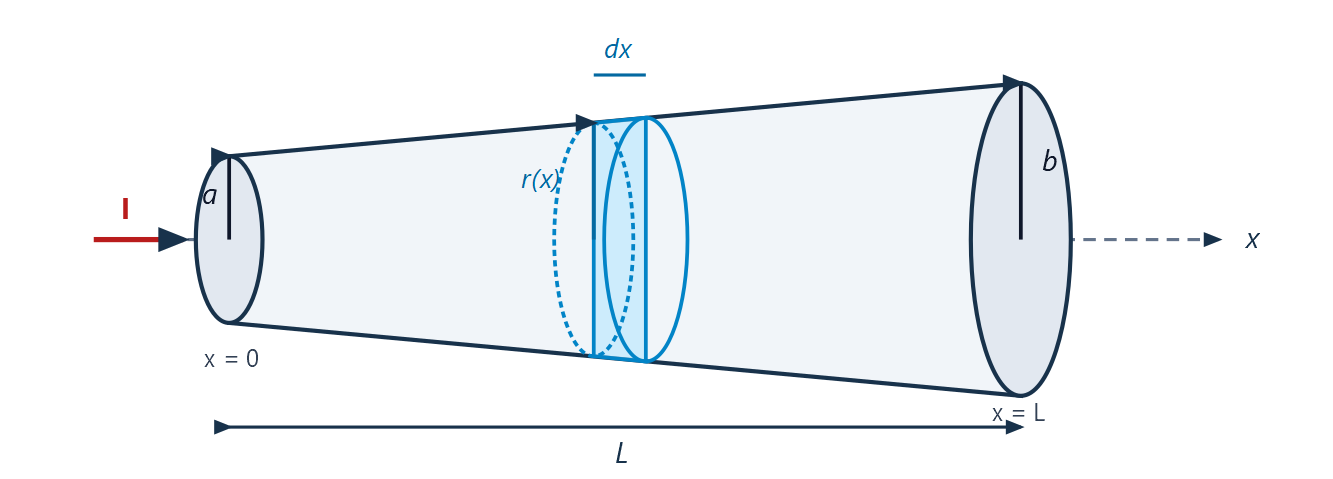
\includegraphics[width=0.72\linewidth]{block_s1_assets/s1-q1-cone.png}\end{center}
  \begin{enumerate}
    \item[(i)] Write the cross-sectional radius $r(x)$ and area $A(x)$ at axial position $x \in [0, L]$, and write the differential resistance $dR$ of an infinitesimal disk slab of thickness $dx$.
    \item[(ii)] Integrate $R_{\rm 1D} = \int_0^L dR$ explicitly to find the resistance predicted by this slice model.
    \item[(iii)] Verify that your formula recovers the elementary uniform-cylinder formula in the limit $b \to a$, and find the electric field magnitude $E(x)$ as a function of $x$ in terms of $I, \rho, a, b, L$.
  \end{enumerate}
\end{enumerate}

\newpage
\section*{Exercise 02 $\cdot$ Mixed Series--Parallel DC Ladder \& Short-Circuit Perturbation \hfill [10 Points $\cdot$ FR]}
An ideal DC voltage source $V_s = 36.0\text{ V}$ supplies a series resistor $R_1 = 6.00\ \Omega$ connected at junction $B$ to two parallel branches: branch 1 contains $R_2 = 18.0\ \Omega$ alone, and branch 2 contains $R_3 = 4.00\ \Omega$ in series with $R_4 = 5.00\ \Omega$. Node $G$ is grounded ($V_G = 0\text{ V}$).
\begin{center}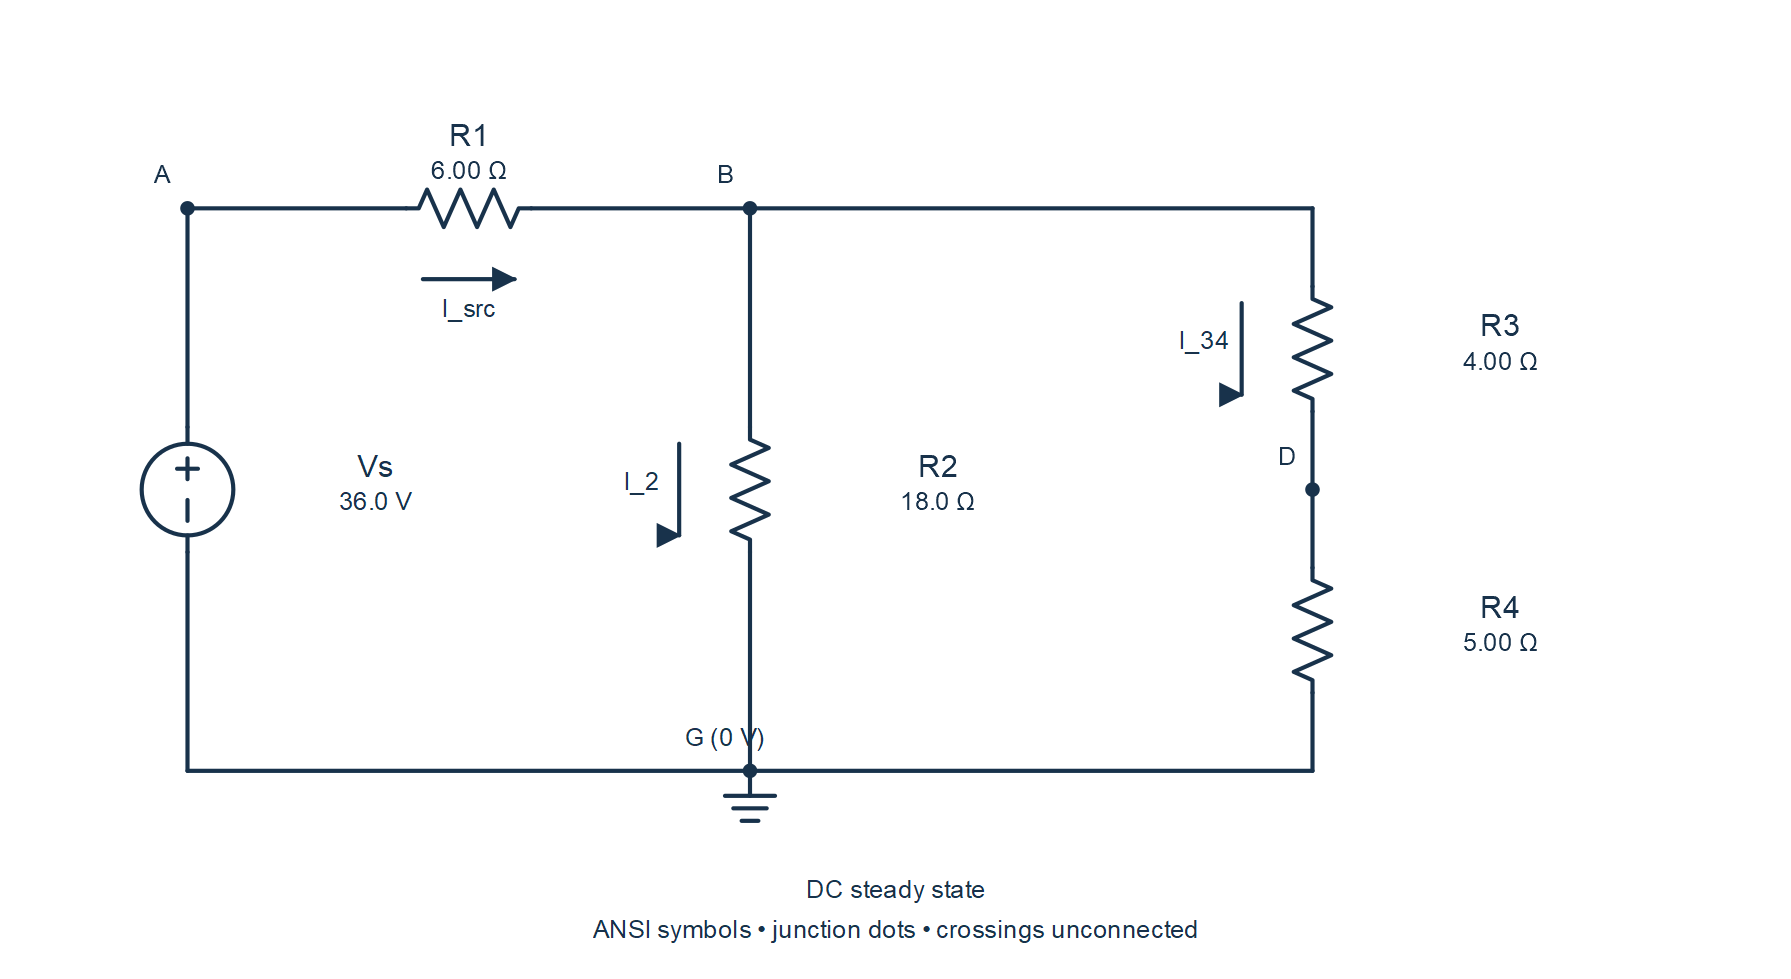
\includegraphics[width=0.75\linewidth]{block_s1_assets/s1-q2-ladder.png}\end{center}
\begin{enumerate}
  \item[(a)] \textbf{Network Reduction [2 pts]:} Calculate the equivalent resistance $R_{BG}$ of the parallel block between node $B$ and ground $G$, and the total equivalent resistance $R_{\text{eq}}$ seen by the $36.0\text{ V}$ source.
  \item[(b)] \textbf{Branch Currents \& Node Potentials [3 pts]:} Determine the source current $I_{\text{src}}$, the node potentials $V_B$ and $V_D$, and the branch currents $I_2$ and $I_{34}$. Verify that $I_2$ and $I_{34}$ satisfy both KCL at node $B$ and the current-divider ratio.
  \item[(c)] \textbf{Power Bookkeeping [2 pts]:} Compute the electrical power dissipated in each of the four resistors ($P_{R_1}, P_{R_2}, P_{R_3}, P_{R_4}$) and verify that $\sum_{k=1}^4 P_{R_k} = P_{\text{source}} = V_s I_{\text{src}}$.
  \item[(d)] \textbf{Topology Perturbation (Shorted Element) [3 pts]:} Suppose a metallic jumper wire accidentally shorts node $B$ directly to node $D$ (so $R_3$ is bypassed, $R_3 \to 0$). Calculate the new equivalent resistance $R_{\text{eq}}'$, the new source current $I_{\text{src}}'$, and the new power $P_{R_4}'$ dissipated in $R_4$. By what factor does $P_{R_4}$ increase?
\end{enumerate}

\newpage
\section*{Exercise 03 $\cdot$ Multi-Source KVL/KCL Network \& Power Direction \hfill [12 Points $\cdot$ FR]}
Three parallel branches connect top junction $A$ to grounded bottom reference node $B$ ($V_B = 0\text{ V}$). Each ideal EMF source has its positive ($+$) terminal oriented upward. Downward reference currents $I_1, I_2, I_3$ are defined from node $A$ toward node $B$ as shown in the Spec v2 schematic below.
\begin{center}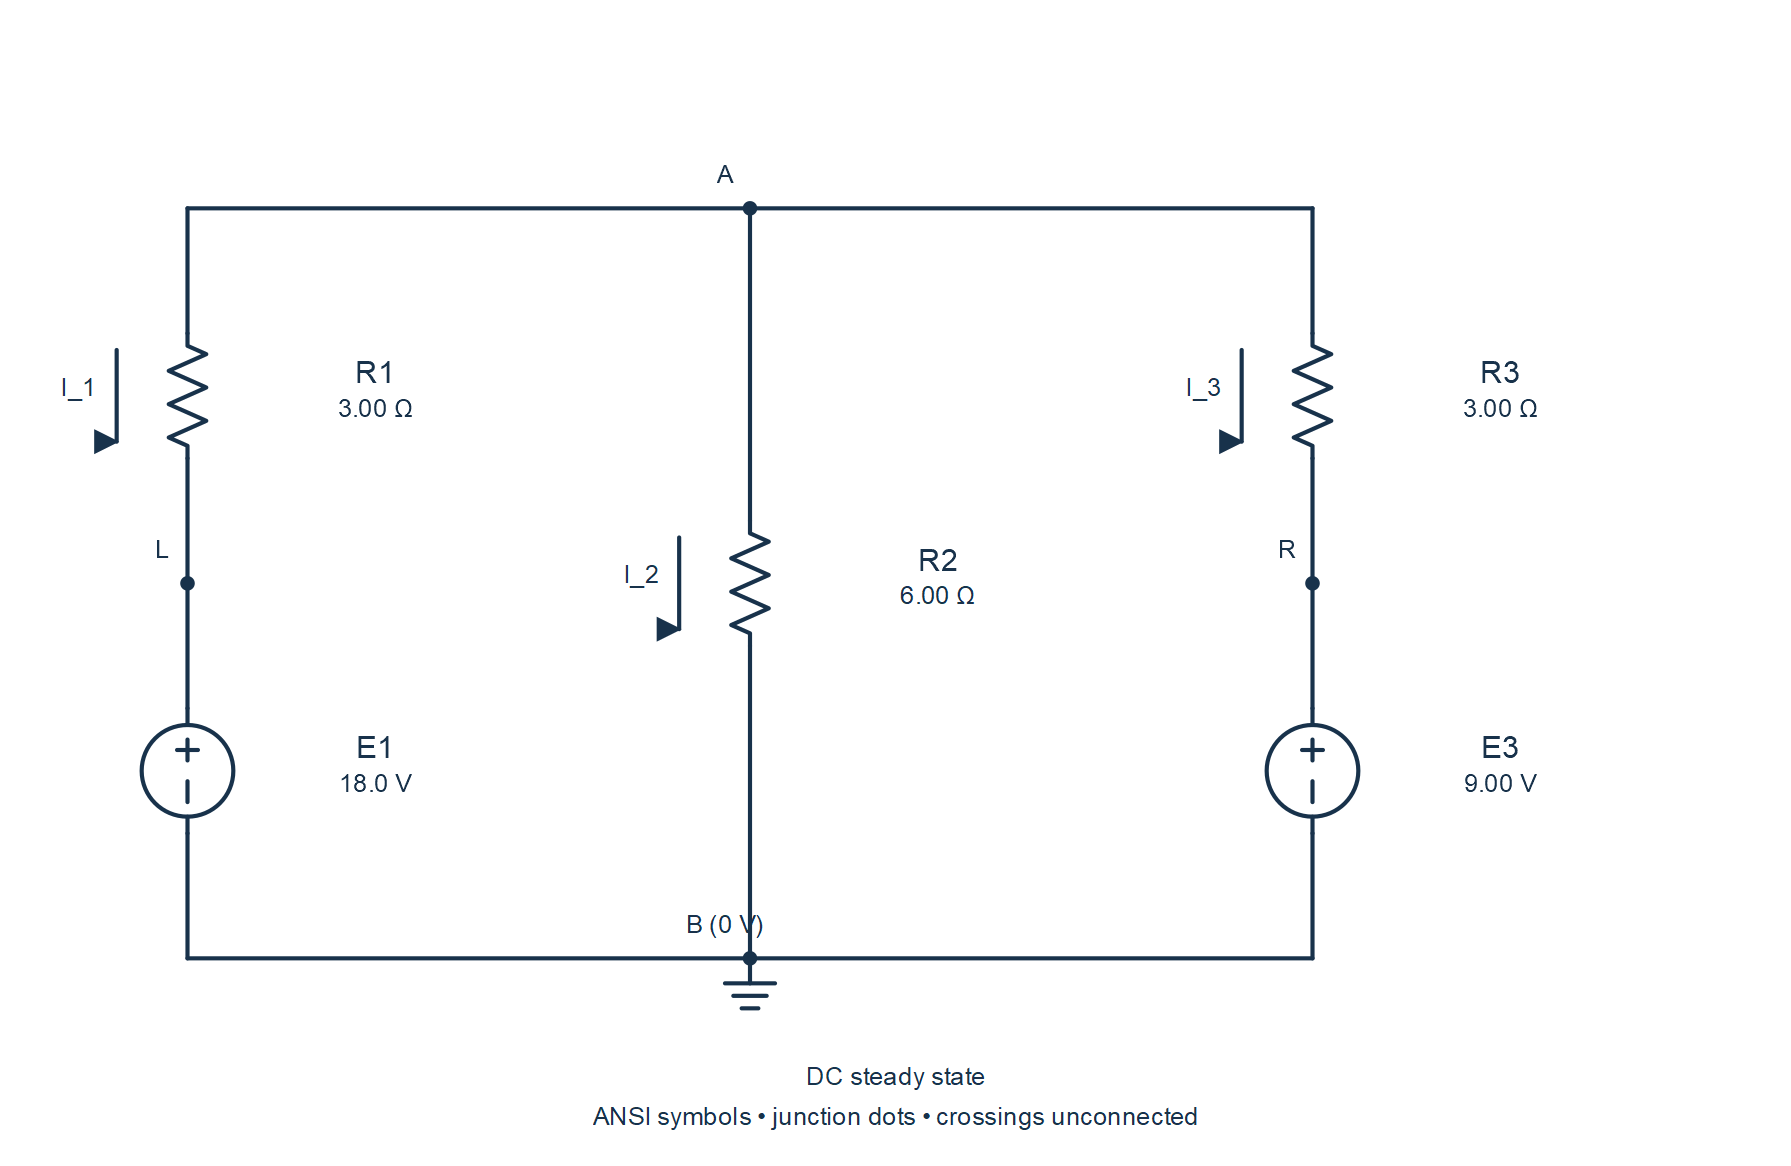
\includegraphics[width=0.76\linewidth]{block_s1_assets/s1-q3-multisource.png}\end{center}
\begin{enumerate}
  \item[(a)] \textbf{KCL \& KVL Formulation [3 pts]:} Write (i) the KCL junction equation at node $A$ in terms of $I_1, I_2, I_3$, (ii) the KVL loop equation around the left mesh (containing $\mathcal{E}_1, R_1, R_2$), and (iii) the KVL loop equation around the right mesh (containing $R_2, R_3, \mathcal{E}_3$).
  \item[(b)] \textbf{Nodal \& Mesh Solution [5 pts]:} Express $I_1, I_2, I_3$ in terms of the single unknown node potential $V_A$, solve for $V_A$, and compute the signed currents $I_1, I_2, I_3$. State the actual physical direction (upward or downward) of current in each branch, and verify that your currents satisfy both KVL equations from part (a).
  \item[(c)] \textbf{Source Power Delivery vs.\ Absorption [4 pts]:} For each EMF source ($\mathcal{E}_1 = 18.0\text{ V}$ and $\mathcal{E}_3 = 9.00\text{ V}$), determine whether the source is \textbf{delivering} electrical power to the circuit or \textbf{absorbing} electrical power (being charged). Calculate both source powers and verify global conservation of energy against total resistor Joule heating $\sum_{k=1}^3 I_k^2 R_k$.
\end{enumerate}

\newpage
\section*{Exercise 04 $\cdot$ Conceptual Cloze \& Maximum Power Transfer Graphs \hfill [10 Points $\cdot$ CLOZE + DRAW]}
\subsection*{Part A: Conceptual Cloze with Word Bank [4 points --- 0.5 pt each]}
\noindent\colorbox{pale}{\parbox{\dimexpr\linewidth-2\fboxsep\relax}{%
\textbf{WORD BANK:} \texttt{electric charge} $\cdot$ \texttt{energy} $\cdot$ \texttt{magnetic flux} $\cdot$ \texttt{smaller than} $\cdot$ \texttt{larger than} $\cdot$ \texttt{opposite to} $\cdot$ \texttt{equal to} $\cdot$ \texttt{$\mathcal{E} - Ir$} $\cdot$ \texttt{$\mathcal{E} + Ir$} $\cdot$ \texttt{open circuit} $\cdot$ \texttt{short circuit} $\cdot$ \texttt{zero}%
}}
\begin{enumerate}
  \item[(a)] Kirchhoff's junction rule (KCL, $\sum I = 0$) is a direct statement of local conservation of \underline{\hspace{2.2in}} at a steady-state node.
  \item[(b)] Kirchhoff's loop rule (KVL, $\sum_{\rm loop} \Delta V = 0$, including source rises and resistor drops) follows from conservation of \underline{\hspace{2.2in}} per unit charge.
  \item[(c)] When any positive resistor $R_{\text{new}}$ is connected in parallel across an existing resistor network, the new equivalent resistance is strictly \underline{\hspace{2.2in}} the smallest individual branch resistance.
  \item[(d)] If solving a KVL/KCL system yields $I_1 = -2.40\text{ A}$, the negative sign means the actual current has magnitude $2.40\text{ A}$ and flows \underline{\hspace{2.2in}} the assumed reference arrow.
  \item[(e)] When a real battery (EMF $\mathcal{E}$, internal resistance $r$) supplies current $I$ out of its positive terminal (discharging), its terminal voltage is \underline{\hspace{2.2in}}.
  \item[(f)] When an external source forces current $I$ \emph{into} the positive terminal of a real battery (charging), its terminal voltage is \underline{\hspace{2.2in}}.
  \item[(g)] An ideal voltmeter has infinite internal resistance and behaves as an \underline{\hspace{2.2in}} when connected in parallel across a circuit element.
  \item[(h)] An ideal ammeter has negligible resistance and behaves like a \underline{\hspace{2.2in}} when inserted in series.
\end{enumerate}

\subsection*{Part B: Draw the Effect \& Calculus of Maximum Power Transfer [6 points --- DRAW + DERIVE]}
A real DC source has open-circuit EMF $\mathcal{E} = 18.0\text{ V}$ and internal resistance $r = 3.00\ \Omega$, and is connected across a variable load resistor $R_L \in [0, 15.0\ \Omega]$.
\begin{enumerate}
  \item[(i)] \textbf{Calculus Proof [2 pts]:} Express $P_L(R_L)=I^2R_L$ in terms of $\mathcal{E}$, $r$, and $R_L$. Differentiate, find and classify the stationary point, then calculate its resistance and peak power.
  \item[(ii)] \textbf{Plot 1 [2 pts]:} On grid (i) below, plot the terminal voltage $V_T$ (\textbf{dependent variable}, vertical axis, in $\text{V}$) vs.\ load current $I$ (\textbf{independent variable}, horizontal axis, in $\text{A}$) from $I = 0$ to $I_{\text{sc}} = 6.00\text{ A}$. Label the open-circuit intercept, the short-circuit intercept, the operating point at $R_L = r$, and the slope.
  \item[(iii)] \textbf{Plot 2 [2 pts]:} On grid (ii) below, plot the load power $P_L$ (\textbf{dependent variable}, vertical axis, in $\text{W}$) vs.\ load resistance $R_L$ (\textbf{independent variable}, horizontal axis, in $\Omega$) for $0 \le R_L \le 15.0\ \Omega$. Mark the peak found in (i) and label the values at $R_L=0$, $6.00\ \Omega$, and $15.0\ \Omega$.
\end{enumerate}
\begin{center}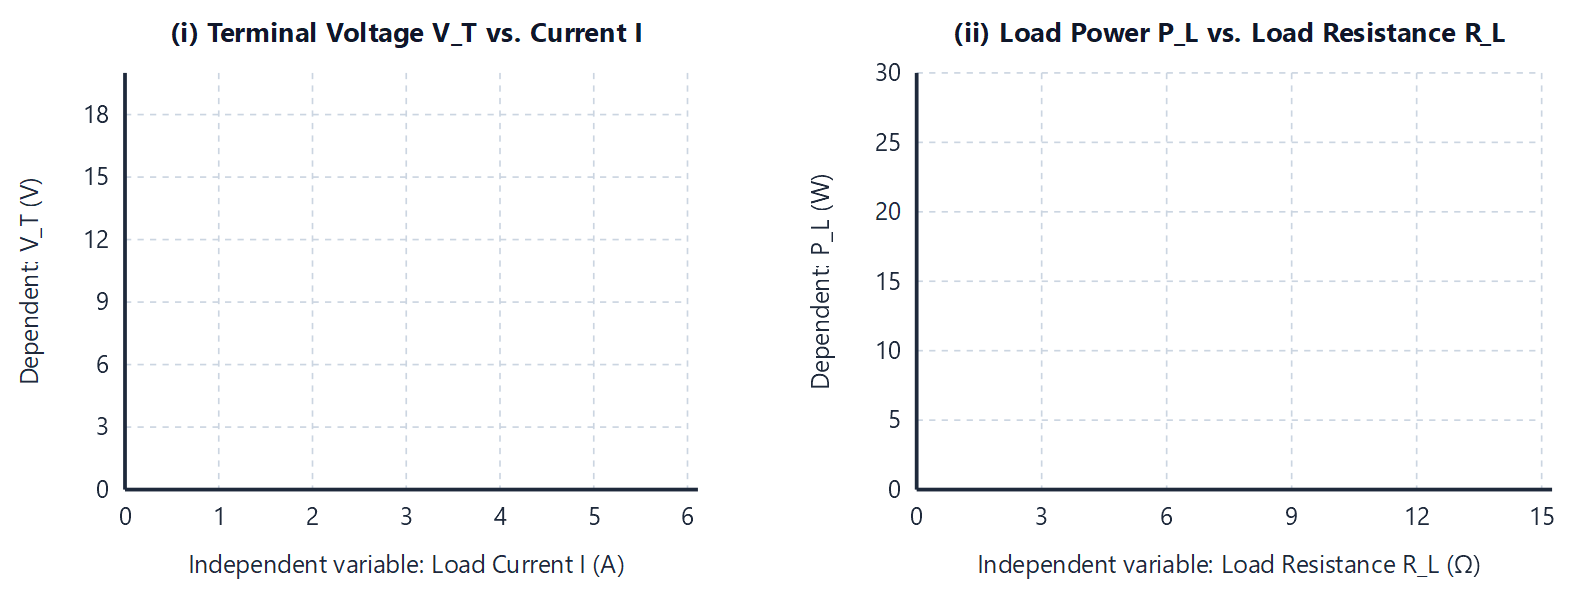
\includegraphics[width=0.96\linewidth]{block_s1_assets/s1-q4-grid-blank.png}\end{center}

\end{document}
